% Section content template for individual Educative lessons
% This file contains the actual content for a specific section
% Generated from Educative API section content

% Section: Activity Diagram for the Chess Game
% Section ID: 6608838909493248
% Section Slug: activity-diagram-for-the-chess-game
% Generated: 2025-12-12T16:11:21.554983

An activity diagram is a great way to visualize the flow of messages from one activity to another in the system. We can create different activity diagrams for our chess game. In this lesson, we will create an activity diagram to show how to play chess.

\subsection{Chess game}\label{tcj3vTybfYmwJbvg1LuZq}
\\
The following states and actions will be involved in this activity diagram.

\subsubsection{States}\label{bZ-uKk9FU8DR8iSfGO008}

\begin{itemize}
\item
\protect\phantomsection\label{USyhdqYx_PgD8i-Qba4MI}
\textbf{Initial state:} The player makes the first move.
\item
\protect\phantomsection\label{zCc3SNjxEZz-rXUWqqwXH}
\textbf{Final state:} Any of the game-over conditions is met.
\end{itemize}

\subsubsection{Actions}\label{ygDZ6rtIxjZYjFIr0Bfr9}
\\
The player initiates a new game. The board appears, and the player takes a turn. The system validates each move and then checks if any game-over conditions (such as checkmate, resignation, forfeit, or draw) have been met. If the game is not over, play continues with the next turn. This process repeats until the system detects a game-over condition and automatically declares the result.
\\
Based on this flow, the activity diagram of the chess game is given below.
\\
We've looked at the activity diagram for our chess game. In the next lesson, we will present the code for our designed classes in some of the most popular programming languages.

\begin{figure}[htbp]
 \centering
 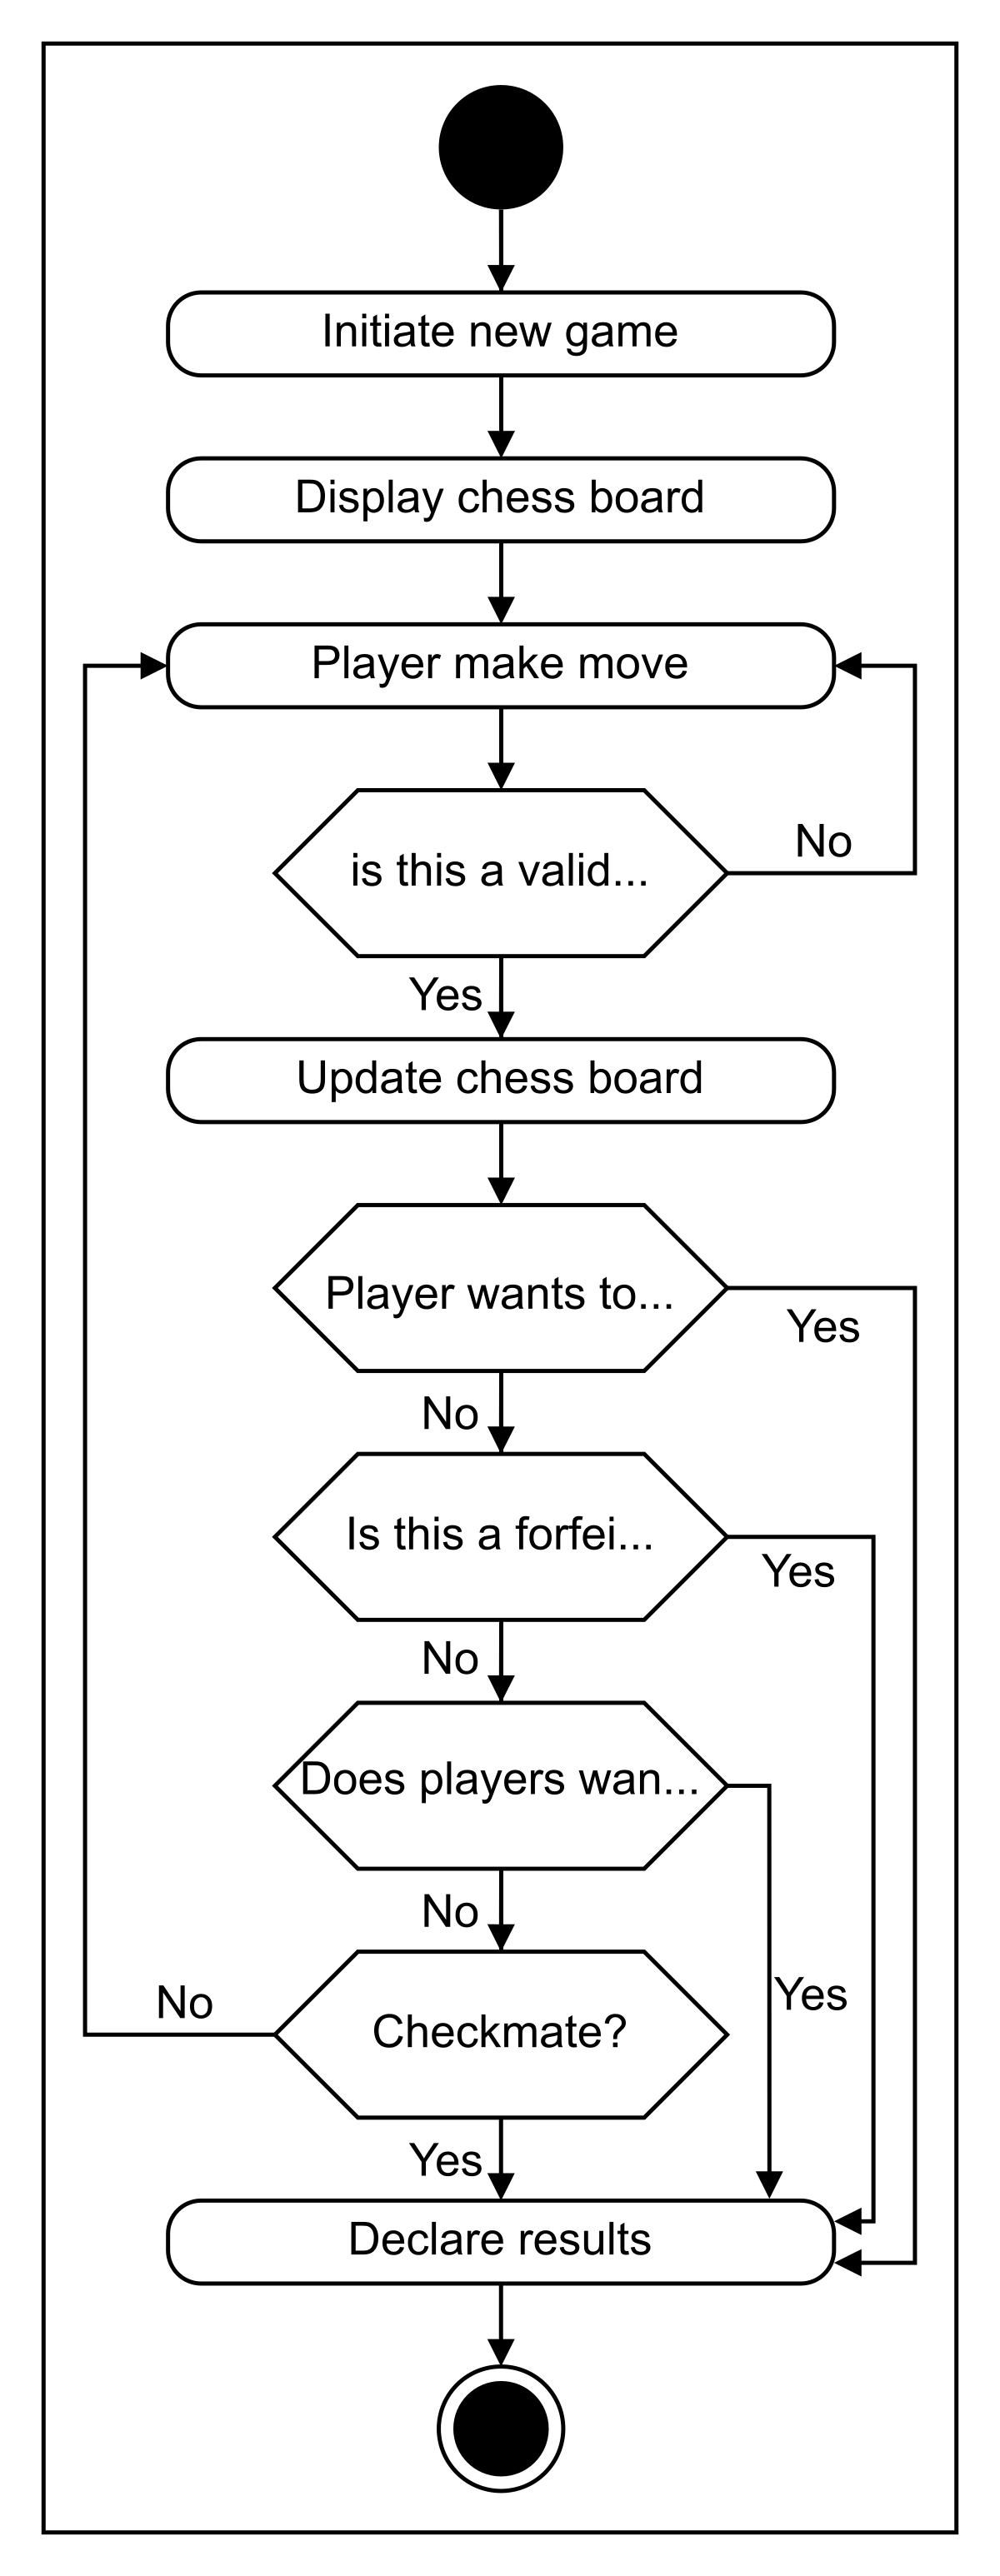
\includegraphics[width=0.5\textwidth]{Images/chapter_17/section_6608838909493248/5263610962903040.png}
 \caption{The activity diagram for an online chess game}
\end{figure}

We've looked at the activity diagram of our chess game. In the next lesson, we will present the code for our designed classes in some of the most popular languages.

% End of section content